\documentclass[12pt]{article}
\usepackage{graphicx}
\usepackage{hyperref}
\usepackage[letterpaper, portrait, margin=0.75in]{geometry}
\usepackage{fancyhdr}
\usepackage{pdfpages}
\usepackage{color}
\usepackage{multicol}
  
\usepackage{charter}
\pagestyle{fancy}
\lhead{PSEC4A datasheet}
%\chead{\thepage}
\rhead{v0.1 ---  2017.4.10}


%\usepackage{lmodern}

\begin{document}
\noindent {\huge{\textbf {PSEC4A}}} \\
\noindent Chip Designer and Document Author: Eric Oberla (KICP UChicago) \\
\noindent Email: ejo@uchicago.edu

%\tableofcontents
%\newpage

\section*{Overview}
\begin{multicols}{2}

  This document provides an overview of the PSEC4A ASIC designed in late 2016 and early 2017 and submitted for fabrication on a MOSIS 0.13~$\mu$m CMOS MPW in February, 2017. The PSEC4A ASIC is intended for the `analog down-conversion' of wide-bandwidth ($\sim$2~GHz) analog signals, achieved through fast sampling (1-11 gigasamples-per-second [GSPS]) followed by a relatively slow digitization and readout process ($\mathcal{O}$100~MHz). Thus, PSEC4A requires a trigger signal to capture the signal-of-interest, either from an external source or generated using the PSEC4A internal discriminators.

  The PSEC4A has 8 signal input channels. Each channel has 1056 samples, which are randomly addressable in blocks of 132 samples. The sampling rate is set by an external clock input, which is locked on-chip using a delay-locked loop (DLL). When successfully locked, one input clock period spans the primary sampling array and the sampling rate is equal to 132*$f$, where $f$ is the input clock frequency.
  
\end{multicols}

\section*{Features}
\begin{itemize}
{\bf
  \item `Fast' and `Slow' DLL modes to allow a wide range of stable sampling rates, from $\sim$1~GSPS to 11~GSPS.
  \item Improved input coupling to extend analog bandwidth
  \item Simultaneous sampling / digitization / readout functionality to reduce dead-time induced latency
  \item Multi-buffering via addressable switched-capacitor banks.
  \item On-chip 10-bit DACs for biases and thresholds
  \item Each channel with a threshold-level discriminator and trigger output pin
  \item 11-bit ramp-compare ADC using on-chip 1.5~GHz clock generator
  \item Can be powered through a single 1.2V supply
}

    
\end{itemize}

\section*{Absolute Maximum ratings}
\begin{center}
\begin{tabular}[b!]{l|p{1.4cm}|p{1.7cm}|p{9cm}}
  \hline
   spec       & max & nominal & comment \\ \hline
   Supply Voltage ($\mathrm{V_{dd}}$) &  1.5 V  & 1.2 V  &   may be possible to increase $\mathrm{AV_{dd}}$ only to increase dynamic range\\ \hline
   IO voltage &  $\mathrm{V_{dd}}$ & 1.2 V & Over/under voltage protection diodes on most pins. ({\bf Not} on signal inputs) \\ \hline
   Signal range voltage & 0-$\mathrm{AV_{dd}}$ & 0.1-1.1~V & about a 1~V usable range

\end{tabular}
\end{center}

\newpage
\section*{I/O Descriptions}
The PSEC4A pinout, as housed in the LQFP128 package, is shown in Figure~\ref{fig:pinout}.

\begin{figure}[t!]
    \begin{center}
      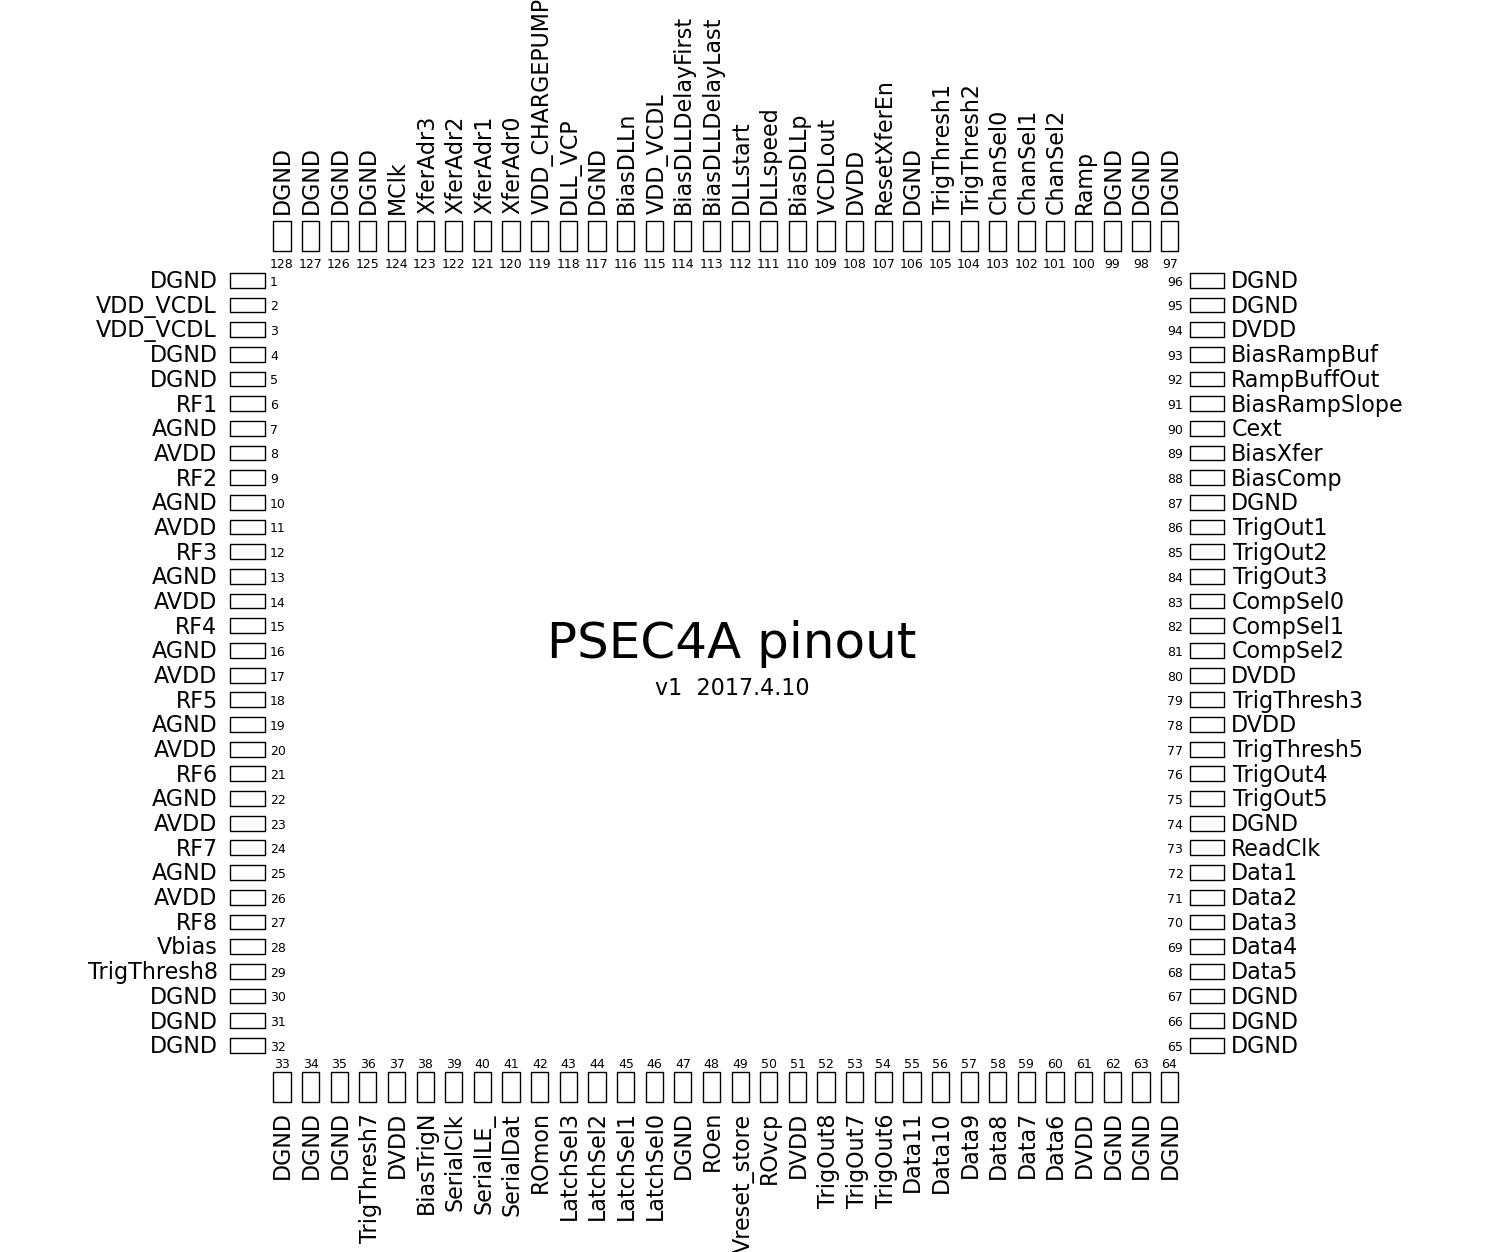
\includegraphics[width=18.3cm]{fig/PSEC4a_pinout_LQFP128.png}
      %\includegraphics[width=15cm]{singlePLL.PNG}

    \end{center}
    \caption{PSEC4A pinout in LQFP128 package}
    \label{fig:pinout}
\end{figure}

\subsection*{Power}
The PSEC4A has four separate +1.2~V $\mathrm{V_{dd}}$ rails and two GND returns.
These can be tied to a single power supply (+1.2~V, GND), but there may (potentially) be
performance benefits when taking care to provide some isolation between these rails. 

\begin{center}
\begin{tabular}[h!]{l|l|p{10cm}}
  \hline
   power rail       & ref &  comment \\ \hline
   $\mathrm{DV_{dd}}$ &  DGND  &  power rail for digital circuitry  \\ \hline
   $\mathrm{V_{dd}VCDL}$ &  DGND  &  power rail for timing generation circuits (VCDL and chip-wide timing drivers) \\ \hline
   $\mathrm{V_{dd}ChargePump}$ &  DGND  &  power rail for DLL feedback circuit \\ \hline
   $\mathrm{AV_{dd}}$ &  AGND  &  power rail for analog circuits and DACs \\ \hline

\end{tabular}
\end{center}

It is likely that using a single PCB GND plane for both DGND and AGND will be satisfactory.

For a conservative design, it is suggested that: 

1) $\mathrm{AV_{dd}}$ be generated by a separate regulator

2) $\mathrm{V_{dd}VCDL}$ be isolated from the $\mathrm{DV_{dd}}$ plane using an appropriate ferrite.

3) $\mathrm{V_{dd}ChargePump}$ be independently generated or further isolated from  $\mathrm{V_{dd}VCDL}$ using a ferrite.
$\mathrm{V_{dd}ChargePump}$ should draw no more than a couple mA.

\subsection*{Serial Interface}

\begin{figure}[h!]
    \begin{center}
      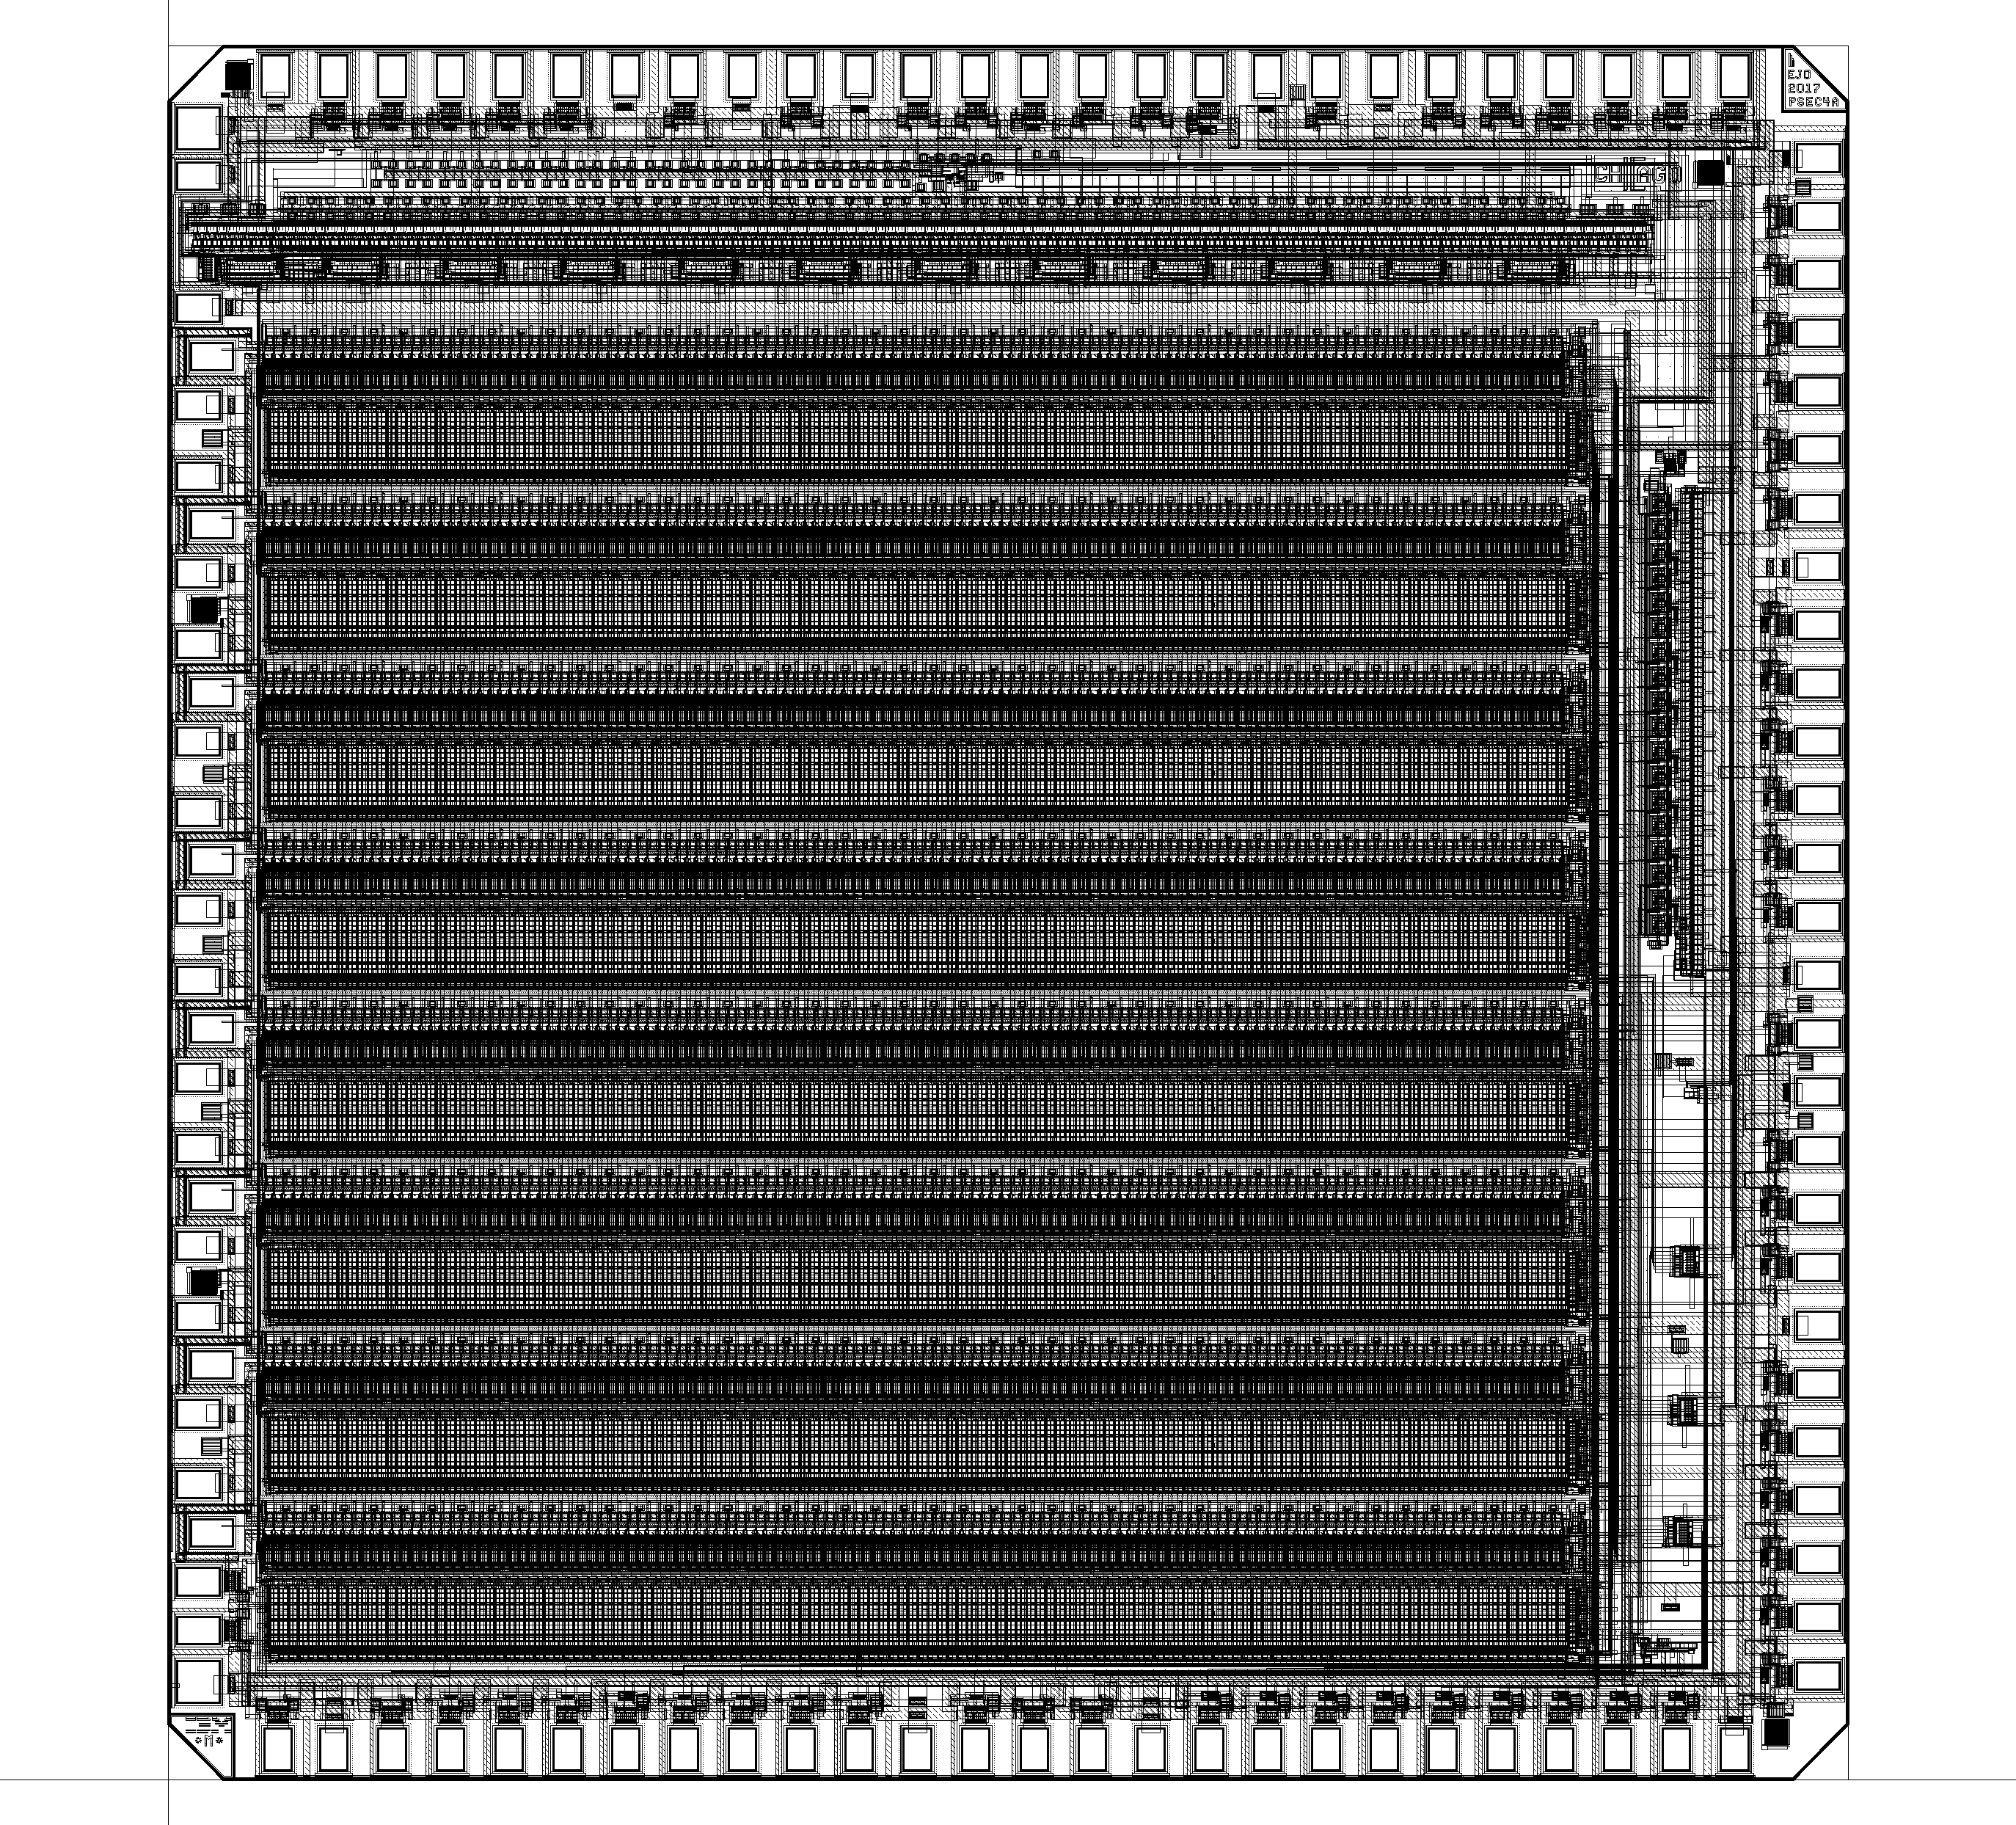
\includegraphics[width=17.5cm]{fig/psec4a_layout_capture}
      %\includegraphics[width=15cm]{singlePLL.PNG}

    \end{center}
    \caption{PSEC4a black-and-white layout capture. The die has 107 pads. The layout has an area of 3800 $\times$ 3920~$\mu$$m^2$.}
    \label{fig:layout}
\end{figure}



%\clearpage
%
%\appendix
%
%\includepdf[pages={1},  offset=0cm -6cm, pagecommand={\section{IPython Notebook: Startup}\label{Appendix0}}]{fig/bootSurf_notebook.pdf}
%\includepdf[pages=2-, offset=0cm -1cm, pagecommand={}]{fig/bootSurf_notebook.pdf}
%
%\includepdf[pages={1}, offset=0cm -2cm, pagecommand={\section{IPython Notebook: Basic Operations}\label{Appendix1}}]{fig/surf_ipython.pdf}
%\includepdf[pages=2-, offset=0cm -2cm, pagecommand={}]{fig/surf_ipython.pdf}
%
%\includepdf[pages={1}, offset=0cm -1cm, pagecommand={\section{IPython Notebook: Tuning DLL feedback trim}\label{Appendix2}}]{fig/vtrimfb_notebook.pdf}
%\includepdf[pages={2-}, offset=0cm -1cm, pagecommand={}]{fig/vtrimfb_notebook.pdf}
%
\end{document}
